

\begin{frame}{Wstęp}

    \begin{block}{Techniki pomiarowe wewnątrz i zewnątrzkomórkowe w neurobiologii}
        \begin{itemize}
            \item różne amplitudy sygnałów
            \item inwazyjność badań
            \item obszar badań 
        \end{itemize}
    \end{block}
    \vspace{-3mm} %5mm vertical space

\begin{columns}
        \column{.55\textwidth}
        \begin{figure}[H]
            \includegraphics[scale=0.5]{ch1/intra-extra.png}  
        \end{figure}

        \column{.4\textwidth}
        \begin{alertblock}{Potencjał czynnościowy}
            \begin{figure}[H]
                \includegraphics[scale=0.25]{ch1/ap.png}
            \end{figure}
        \end{alertblock}

    \end{columns}


    
\end{frame}

\begin{frame}{Kierunki rozwoju współczesnych systemów pomiarowych i matryc mikroelektrodowych}
    \vspace{-5mm} %5mm vertical space

    \begin{columns}[t]
        \column{.3\textwidth}
        \begin{figure}[H]
            \includegraphics[scale=0.35]{ch2/neuropixel10.png}  
        \end{figure}

        \column{.3\textwidth}
        \begin{figure}[H]
            \includegraphics[scale=0.35]{ch2/argo.jpeg}  
        \end{figure}

        \column{.35\textwidth}
        \begin{figure}[H]
            \includegraphics[scale=0.2]{ch2/masm64Dsharp.png}
        \end{figure}

        \begin{figure}[H]
            \includegraphics[scale=0.25]{ch2/utahArr.png}
        \end{figure}

    \end{columns}


\end{frame}

\begin{frame}{Zakresy amplitud i częstotliwości sygnałów neuronowych}
    \begin{columns}
        \column{.48\textwidth}
        \begin{figure}[H]
            \includegraphics[scale=0.2]{ch1/brain.jpg}
          \end{figure}
          \begin{block}{Metody rejestracji}
            \begin{itemize}
                \item LFP -- Local Field Potential
                \item AP --  Action Potential
                \item ECoG -- Electrocorticography
                \item EEG -- Electroencephalography
            \end{itemize}
        \end{block}


        \column{.48\textwidth}
        \begin{figure}[H]
            \centering
            \includegraphics[scale=1.0]{ch1/lfp_ap_spectrum}  
            \end{figure}	
    \end{columns}
    
\end{frame}



\begin{frame}{Kanał rejestracji neuronowej z wykorzystaniem elektrod zewnątrzkomórkowych}
\vspace{-1em}
    \begin{columns}
        \column{.48\textwidth}
        \begin{figure}[H]
            \centering
            \includegraphics[scale=0.25]{ch2/chemNeuroInterface.png} 

        \end{figure}
        \begin{figure}[H]
            \centering
            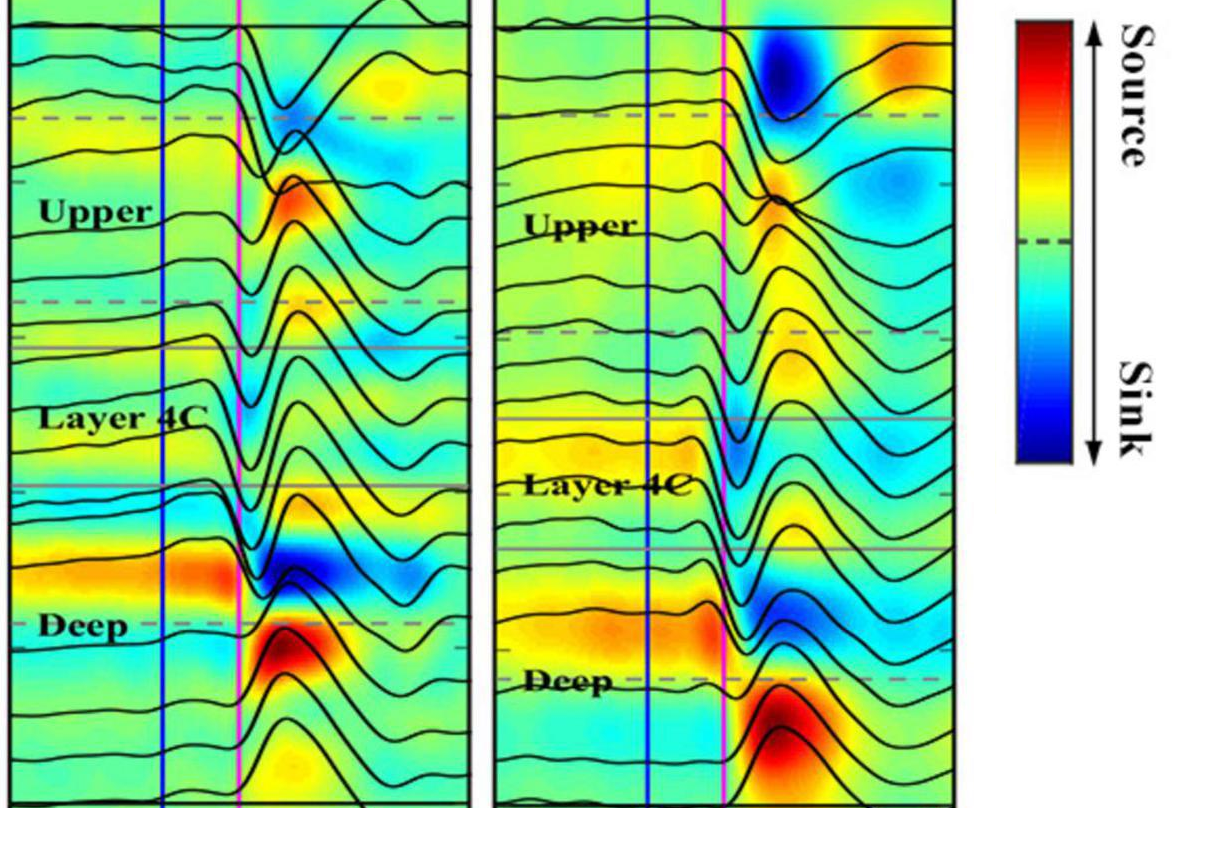
\includegraphics[scale=0.25]{ch1/lfp.png} 

          \end{figure}

        \column{.48\textwidth}
        \begin{block}{Wymagania stawiane interfejsom neuroelektronicznym umożliwiającym rejestrację sygnałów LFP i AP}
            \begin{itemize}
                \item Offset stały na styku elektrody -- do $\SIrange{1}{2}{\volt}$ 
                \item Szumy $<\SI{5}{\micro\volt}$ dla pasma LFP i AP
                \item Liniowość rejestrowanego sygnału
                \item Pobór mocy -- limit ogrzewania tkanki mózgowej --  mniej niż  $\SI{1}{\degreeCelsius}$ 
                \item Zróżnicowane sygnały: amplituda do $\SI{10}{\milli\volt_{pp}}$ dla LFP i od  $\SI{50}{\micro\volt}$ dla AP
                \item Skalowalność systemu -- tysiące kanałów dla przyszłych systemów
            \end{itemize}
        \end{block}
        % Schemat typowego kanału rejestracji neuronowej i modelu elektrycznego interfejsu tkanka-mikroelektroda: 
        % $Z_{CPA}$ -- element o stałej fazie, 
        % $R_{CT}$ -- rezystancja dla przepływającego prądu przez elektrodę,  
        % $R_{SP}$ -- rezystancja rozproszona elektrolitu, 
        % $V_{HC}$ -- potencjał w interfejsie elektroda -- tkanka. 
 
    \end{columns}
\end{frame}


\begin{frame}{Sprzężenie zmiennoprądowe}
    \begin{columns}
        \column{.48\textwidth}

    \begin{figure}[H]
        \centering
        \includegraphics[scale=0.75]{ch2/conceptAC_Harrison.pdf} 
    \end{figure}
    \column{.48\textwidth}
    \begin{alertblock}{Wyzwania zwiazane z sprzęzeniem AC}
        \begin{itemize}
            \item Niska dolna częstotliwość graniczna rzędu~$\SI{\sim 1}{\hertz}$ 
            \item Pojemności w technologi CMOS są rzędu $\SI{}{\femto\farad\per\micro\metre\squared}$
            \item Rezystancja sprzężenia zwrotnego w zakresie $\SI{}{\tera\ohm}$
        \end{itemize}
    \end{alertblock}
    \begin{exampleblock}{Zalety}
        \begin{itemize}
            \item Usunięcie składowej stałej od elektrody niezależnie od jej wartości
            \item Wydajność szumowa i poboru mocy
        \end{itemize}
    \end{exampleblock}
\end{columns}

\end{frame}



\begin{frame}{Sprzężenie stałoprądowe}
    \begin{columns}
        \column{.48\textwidth}
        \begin{figure}[H]
            \centering
            \includegraphics[scale = 0.5]{ch2/dc_coupling.pdf}
        \end{figure}

    \column{.48\textwidth}
    \begin{alertblock}{Wyzwania zwiazane z sprzęzeniem DC}
        \begin{itemize}
            \item Duża wrażliwość na offset
            \item Pobór mocy
        \end{itemize}
    \end{alertblock}
    \begin{exampleblock}{Zalety}
        \begin{itemize}
            \item Brak konieczności używania dużych rezystancji w pętli sprzężenia zwrotnego
        \end{itemize}

        \begin{figure}[H]
            \centering
            \includegraphics[scale=0.5]{ch2/dc-integrator.pdf} 
        \end{figure}

    \end{exampleblock}
\end{columns}

\end{frame}


